\documentclass[noinstructornotes]{ximera}
%handout:  for handout version with no solutions or instructor notes
%handout,instructornotes:  for instructor version with just problems and notes, no solutions
%noinstructornotes:  shows only problem and solutions

%% handout
%% space
%% newpage
%% numbers
%% nooutcomes

%I added the commands here so that I would't have to keep looking them up
%\newcommand{\RR}{\mathbb R}
%\renewcommand{\d}{\,d}
%\newcommand{\dd}[2][]{\frac{d #1}{d #2}}
%\renewcommand{\l}{\ell}
%\newcommand{\ddx}{\frac{d}{dx}}
%\everymath{\displaystyle}
%\newcommand{\dfn}{\textbf}
%\newcommand{\eval}[1]{\bigg[ #1 \bigg]}

%\begin{image}
%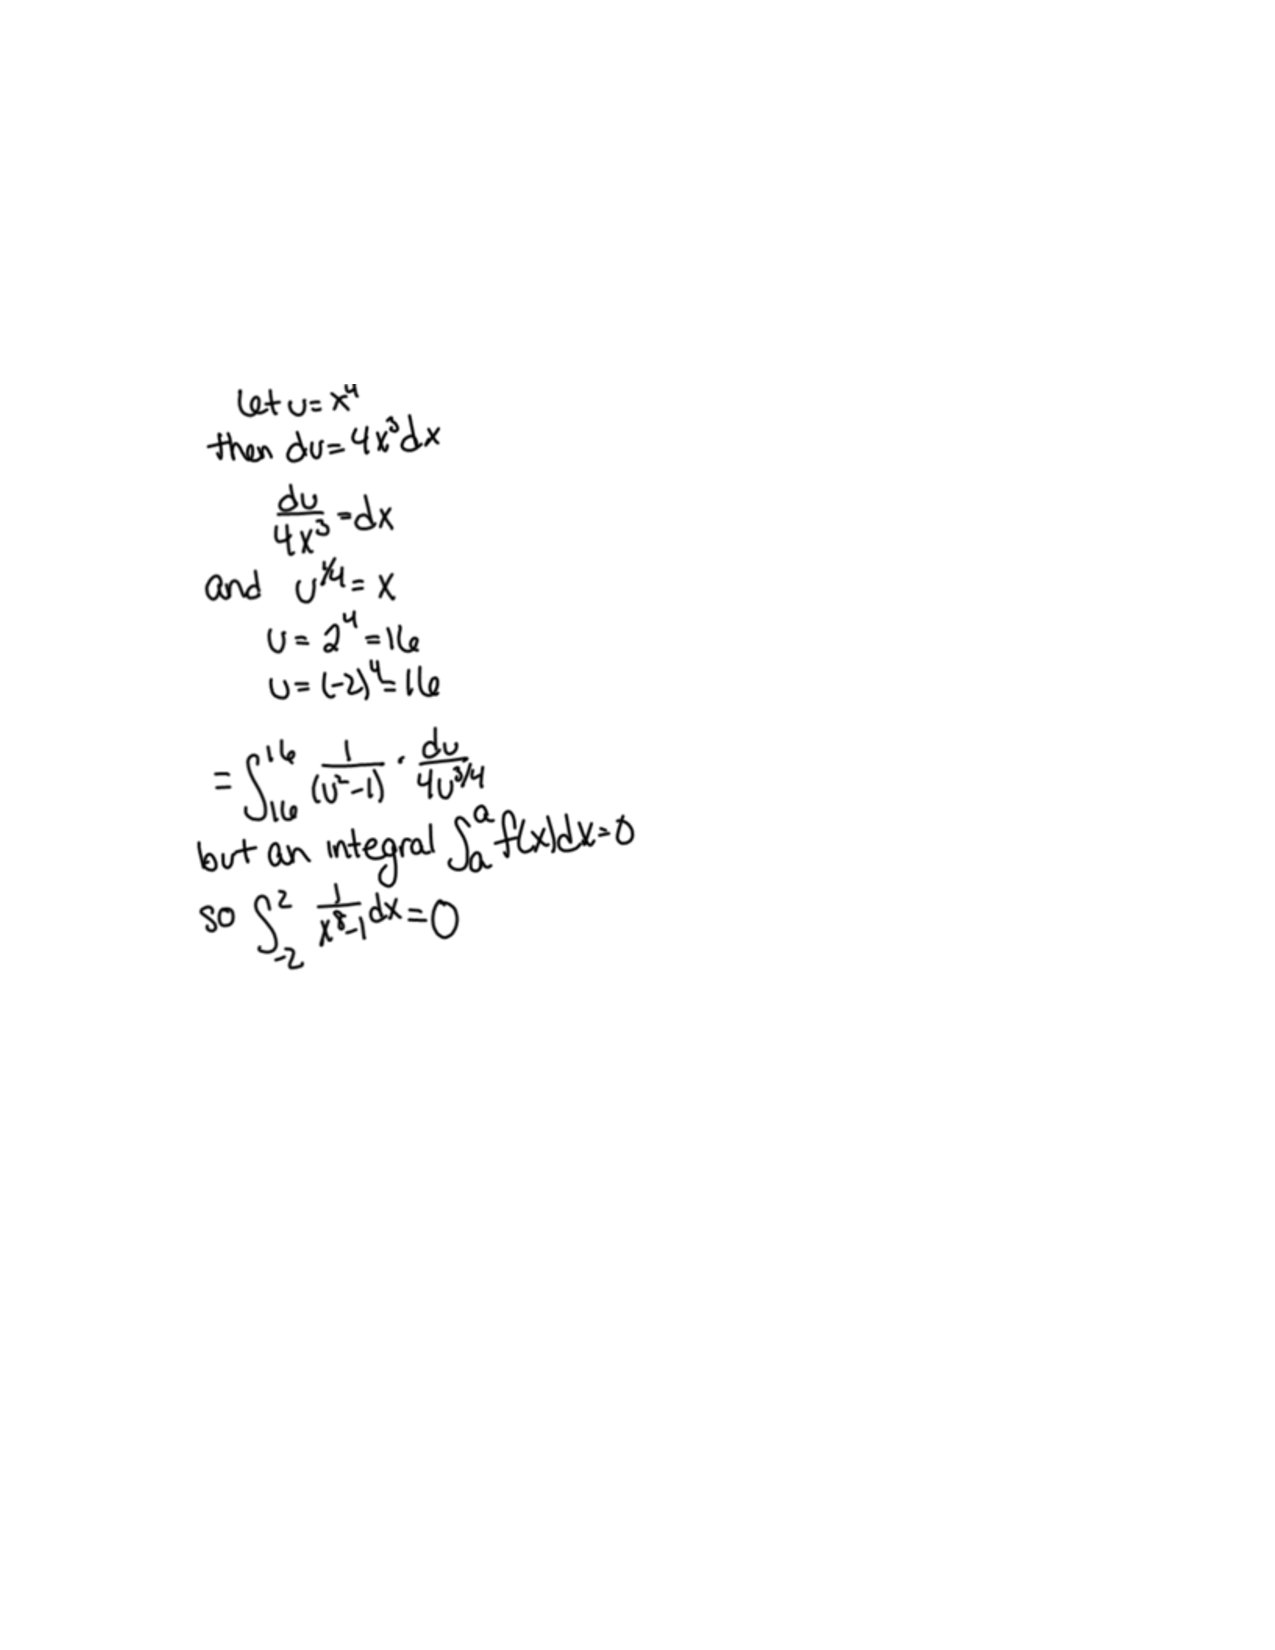
\includegraphics[trim= 170 420 250 180]{Figure1.pdf}
%\end{image}

%add a ``.'' below when used in a specific directory.
\newcommand{\RR}{\mathbb R}
\renewcommand{\d}{\,d}
\newcommand{\dd}[2][]{\frac{d #1}{d #2}}
\renewcommand{\l}{\ell}
\newcommand{\ddx}{\frac{d}{dx}}
\newcommand{\dfn}{\textbf}
\newcommand{\eval}[1]{\bigg[ #1 \bigg]}

\usepackage{multicol}

\renewenvironment{freeResponse}{
\ifhandout\setbox0\vbox\bgroup\else
\begin{trivlist}\item[\hskip \labelsep\bfseries Solution:\hspace{2ex}]
\fi}
{\ifhandout\egroup\else
\end{trivlist}
\fi} %% we can turn off input when making a master document

\title{Recitation \# 4: Volume by Shells \& Length of Curves - Solutions}  

\begin{document}
\begin{abstract}		\end{abstract}
\maketitle



\begin{comment}
\section{Warm up:}

	\begin{freeResponse}
	
	\end{freeResponse}
	
\begin{instructorNotes}

\end{instructorNotes}
\end{comment}







\section{Group work:}



%problem 1
\begin{problem}
Set up an integral that will compute the volume of the solid generated by revolving the region bounded by the curves $y=x^2-6x+13$ (i.e. $x = 3 \pm \sqrt{y-4}$) and $y=3x-1$ about:

\begin{image}
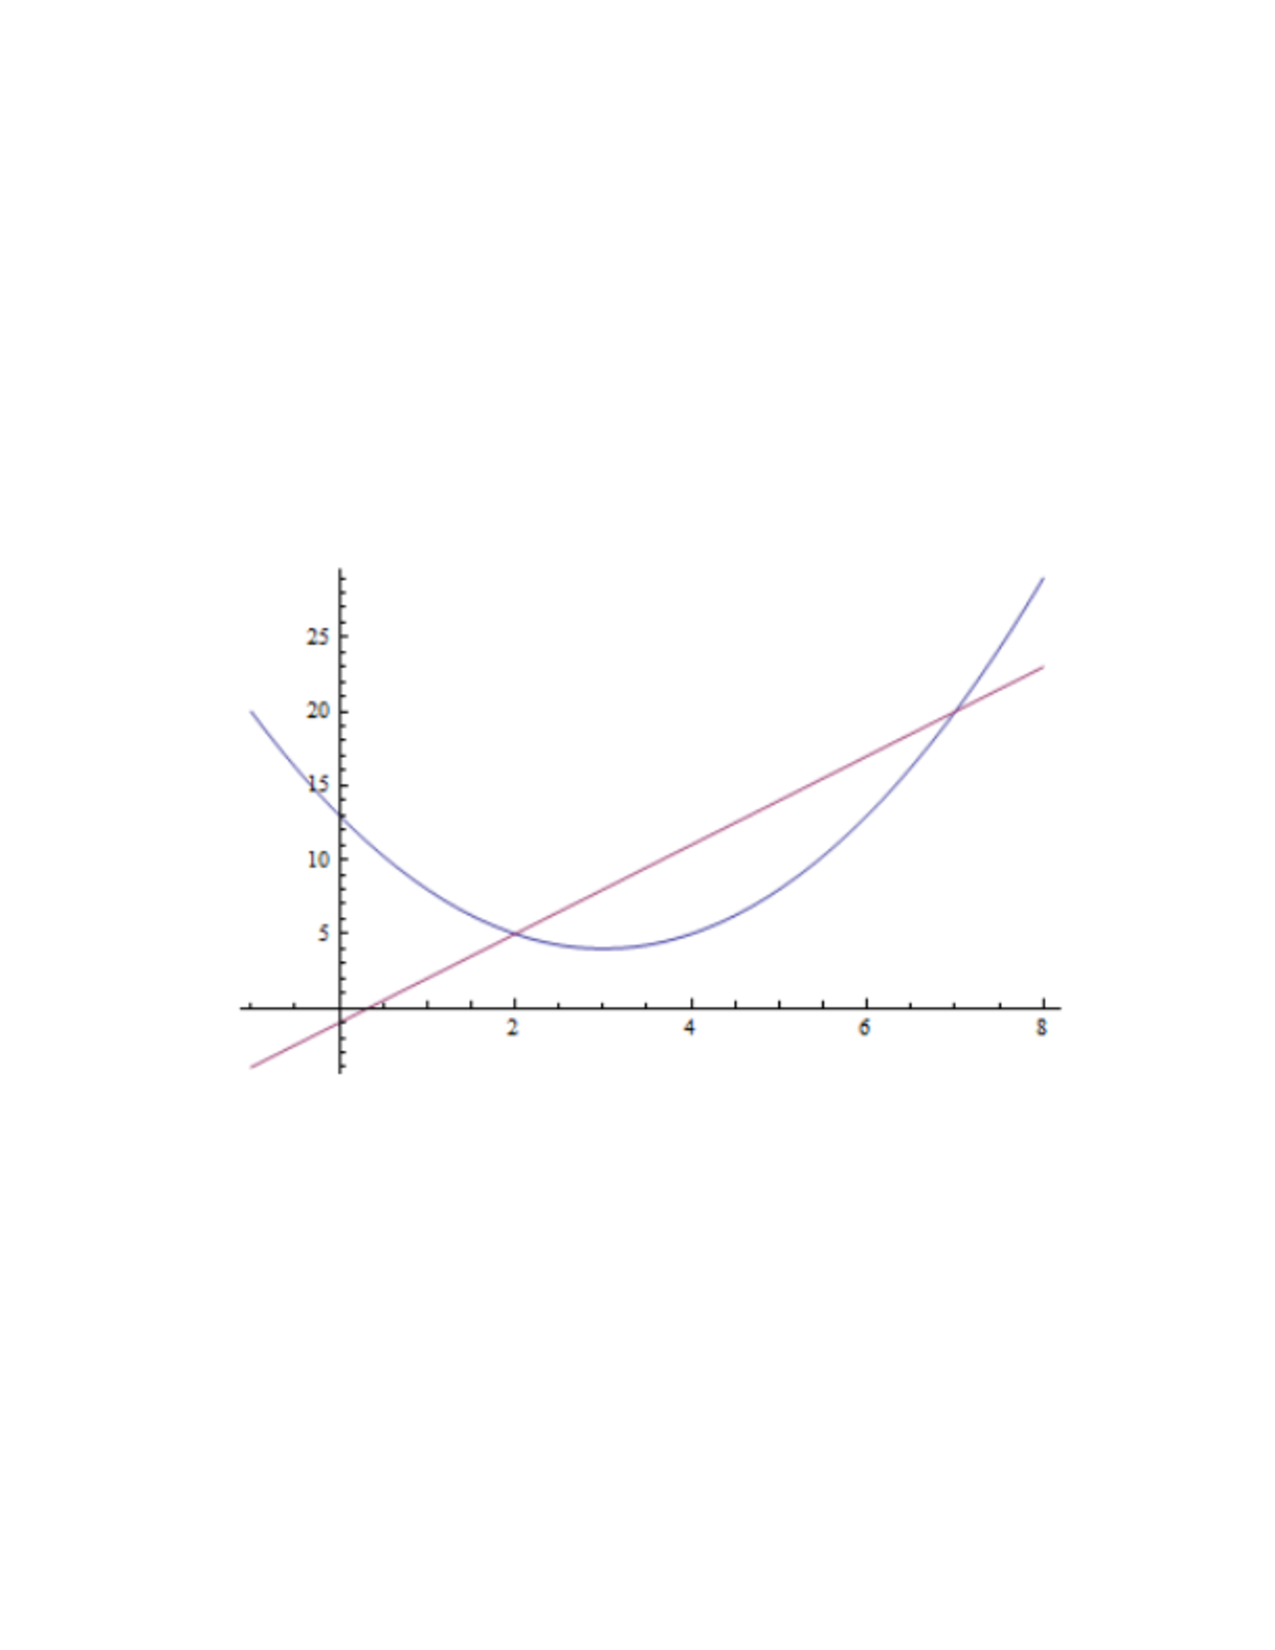
\includegraphics[trim= 170 270 150 280, scale=0.8]{Figure6-4-1.pdf}
\end{image}

Use both the washer method as well as the shell method for each problem.  
Which method would you prefer for each problem?  Why?

	\begin{enumerate}
		\item  the $x$-axis
		\begin{freeResponse}
		First, we need to find the points where the curves intersect
			\begin{align*}
			x^2 - 6x + 13 &= 3x - 1  \\
			x^2 - 9x + 14 &= 0  \\
			(x-2)(x-7) &= 0  \\
			x &= 2, 7  \\
			(2,5&), (7,20).
			\end{align*}
		As we will see later, we also need to locate the vertex of the parabola $x^2 - 6x + 13$.  
		So we complete the square
			\begin{align*}
			y &= x^2 - 6x + 13  \\
			&= (x^2 - 6x \, {\color{red} + \, 9}) + 13 \, {\color{red} - \, 9}  \\
			&= (x-3)^2 + 4.
			\end{align*}
		So the vertex of the parabola is $(3,4)$.  
		
		\begin{image}
		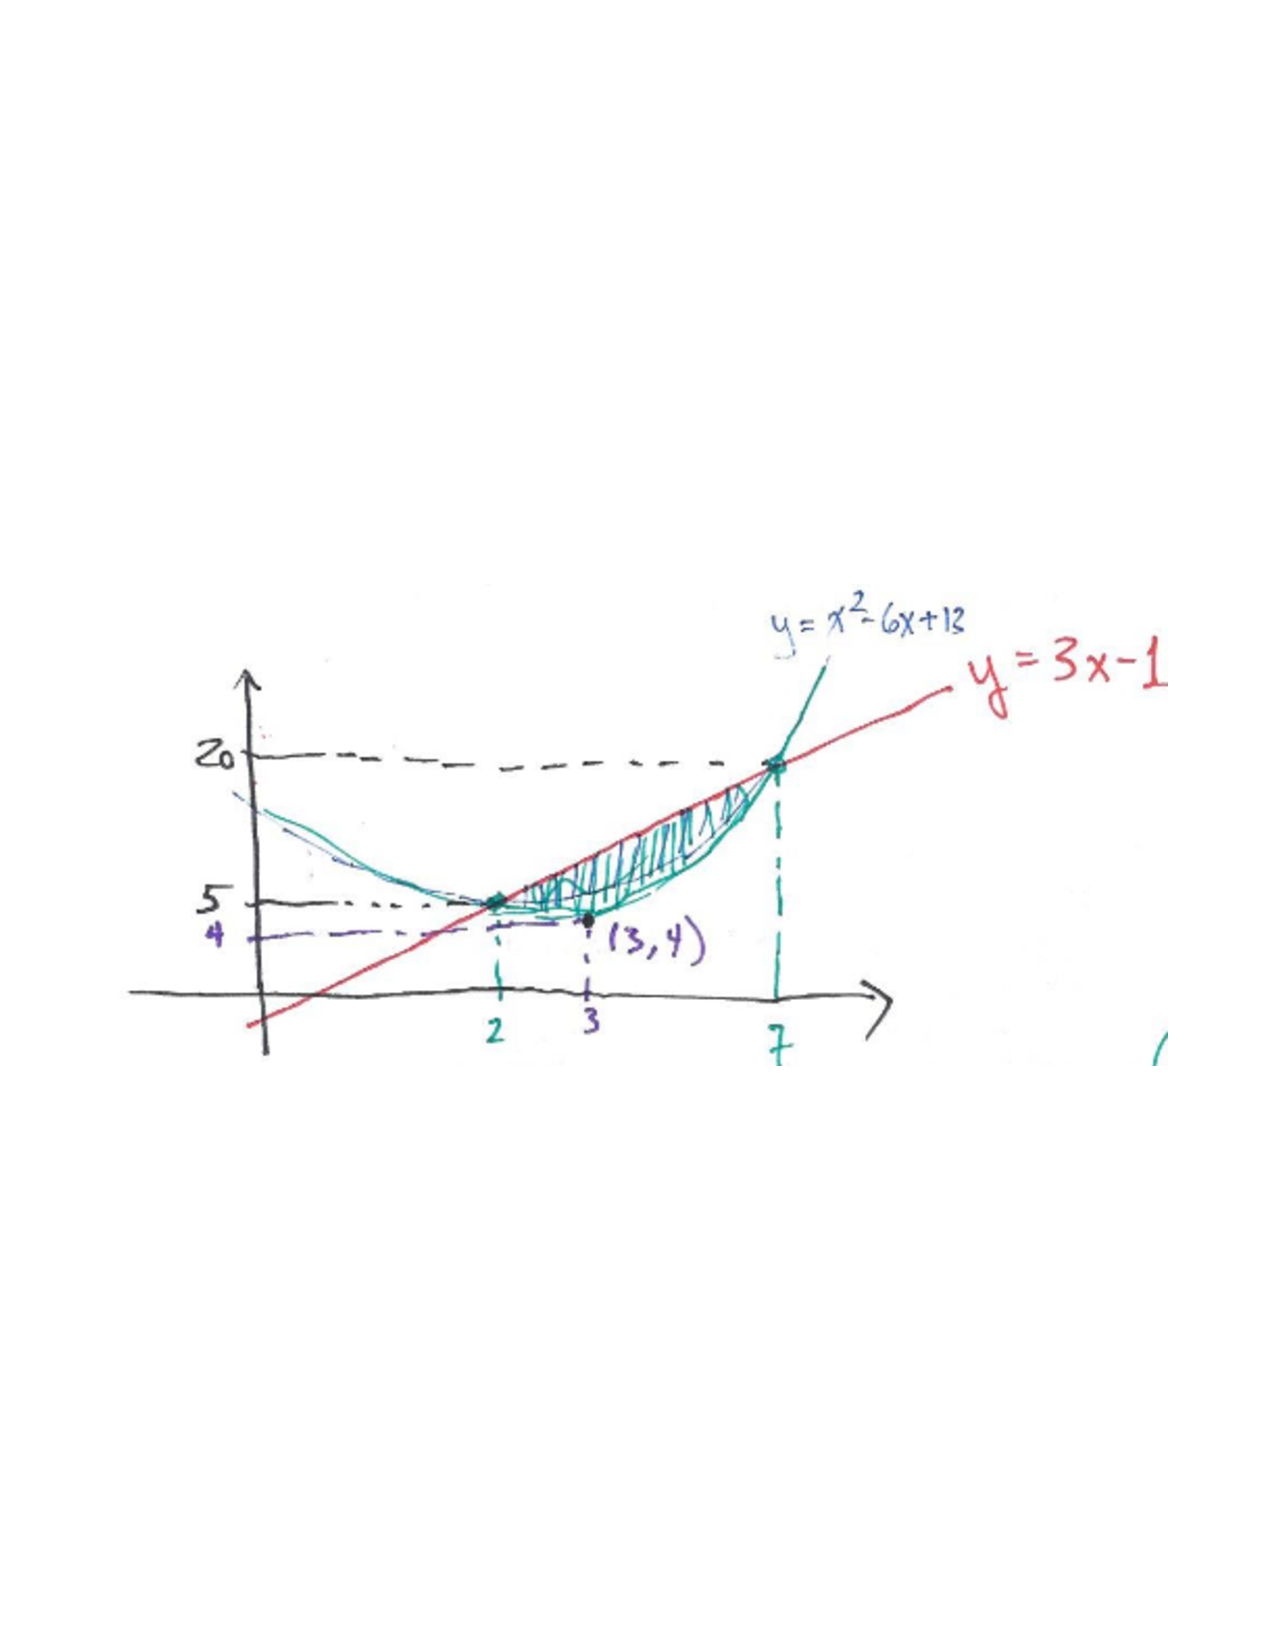
\includegraphics[trim= 170 270 150 280, scale=0.8]{Figure6-4-2.pdf}
		\end{image}

		{\bf Washers: }  For washers, the cross-sections must be \dfn{perpendicular} to the axis of rotation.  
		So here we integrate along the $x$-axis.  
		We have that
			\begin{align*}
			r_{out} &= 3x-1 \\
			r_{in} &= x^2 - 6x +13
			\end{align*}
		and
			\[
			\text{{\color{red} Volume of the region}} = \pi \int_2^7 \left[ (3x-1)^2 - (x^2-6x+13)^2 \right] \d x.
			\]
			
		\begin{image}
		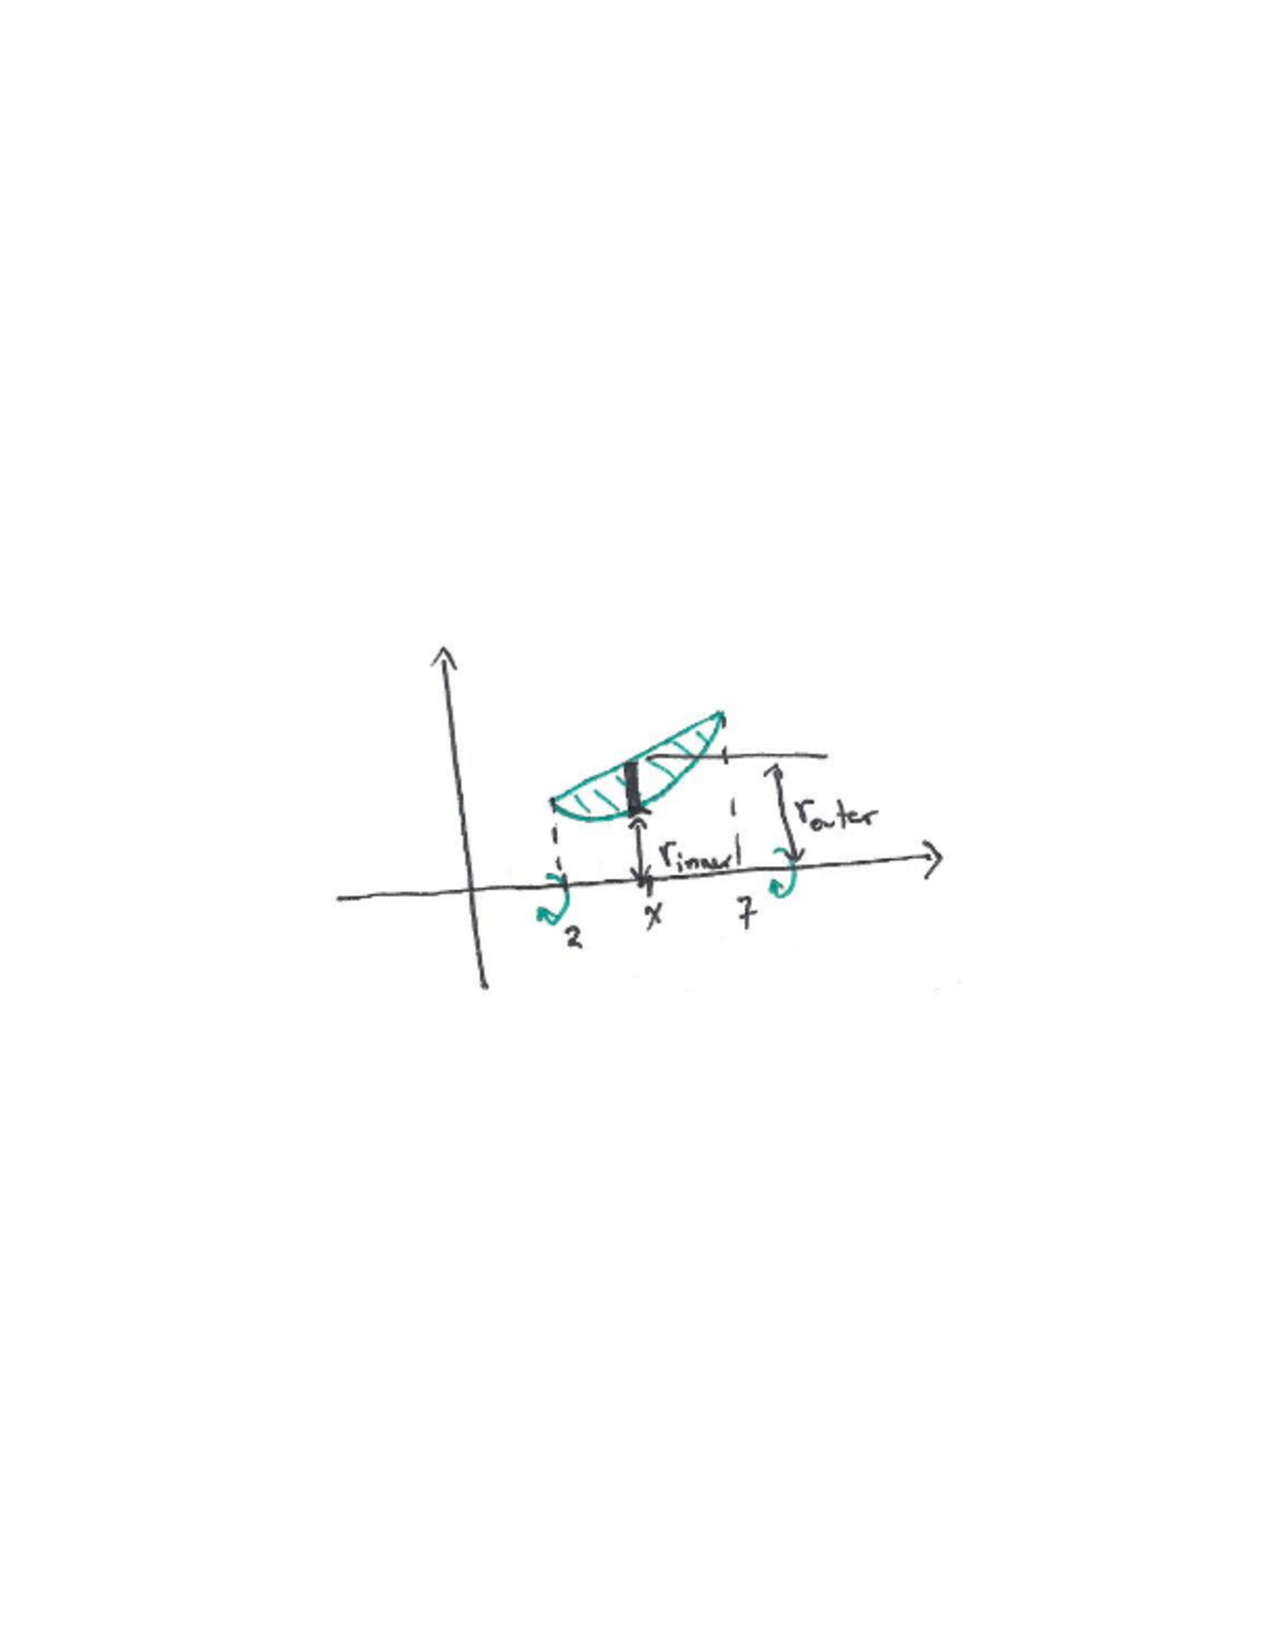
\includegraphics[trim= 200 320 150 310, scale=0.8]{Figure6-4-3.pdf}
		\end{image}
		
		{\bf Shells: }
		For shells, the cross-sections must be \dfn{parallel} to the axis of rotation.  
		So here we integrate along the $y$-axis, $5 \leq y \leq 20$.  
		But we have a problem, namely the ``bottom" of each cross-section changes at $y=5$ due to the shape of the region (see the picture below).
		So we have two different cases:
			\begin{enumerate}
			\item[(1)]  For $4 \leq y \leq 5$
				\begin{align*}
				h &= (3+\sqrt{y-1}) - (3-\sqrt{y-1}) = 2\sqrt{y-1}  \\
				r &= y
				\end{align*}
				
			\item[(2)]  For $5 \leq y \leq 20$
				\begin{align*}
				h &= (3+\sqrt{y-1}) - \left( \frac{1}{3} (y+1) \right)  \\
				r &= y.
				\end{align*}
			\end{enumerate}
		Thus
			\[
			V = \int_4^{20} 2 \pi r h \d y = 2\pi \left[ \int_4^5 y \cdot 2\sqrt{y-1} \d y + \int_5^{20} y \left( (3 + \sqrt{y+1}) - \frac{1}{3}(y+1) \right) \d y \right]
			\]
		
		\begin{image}
		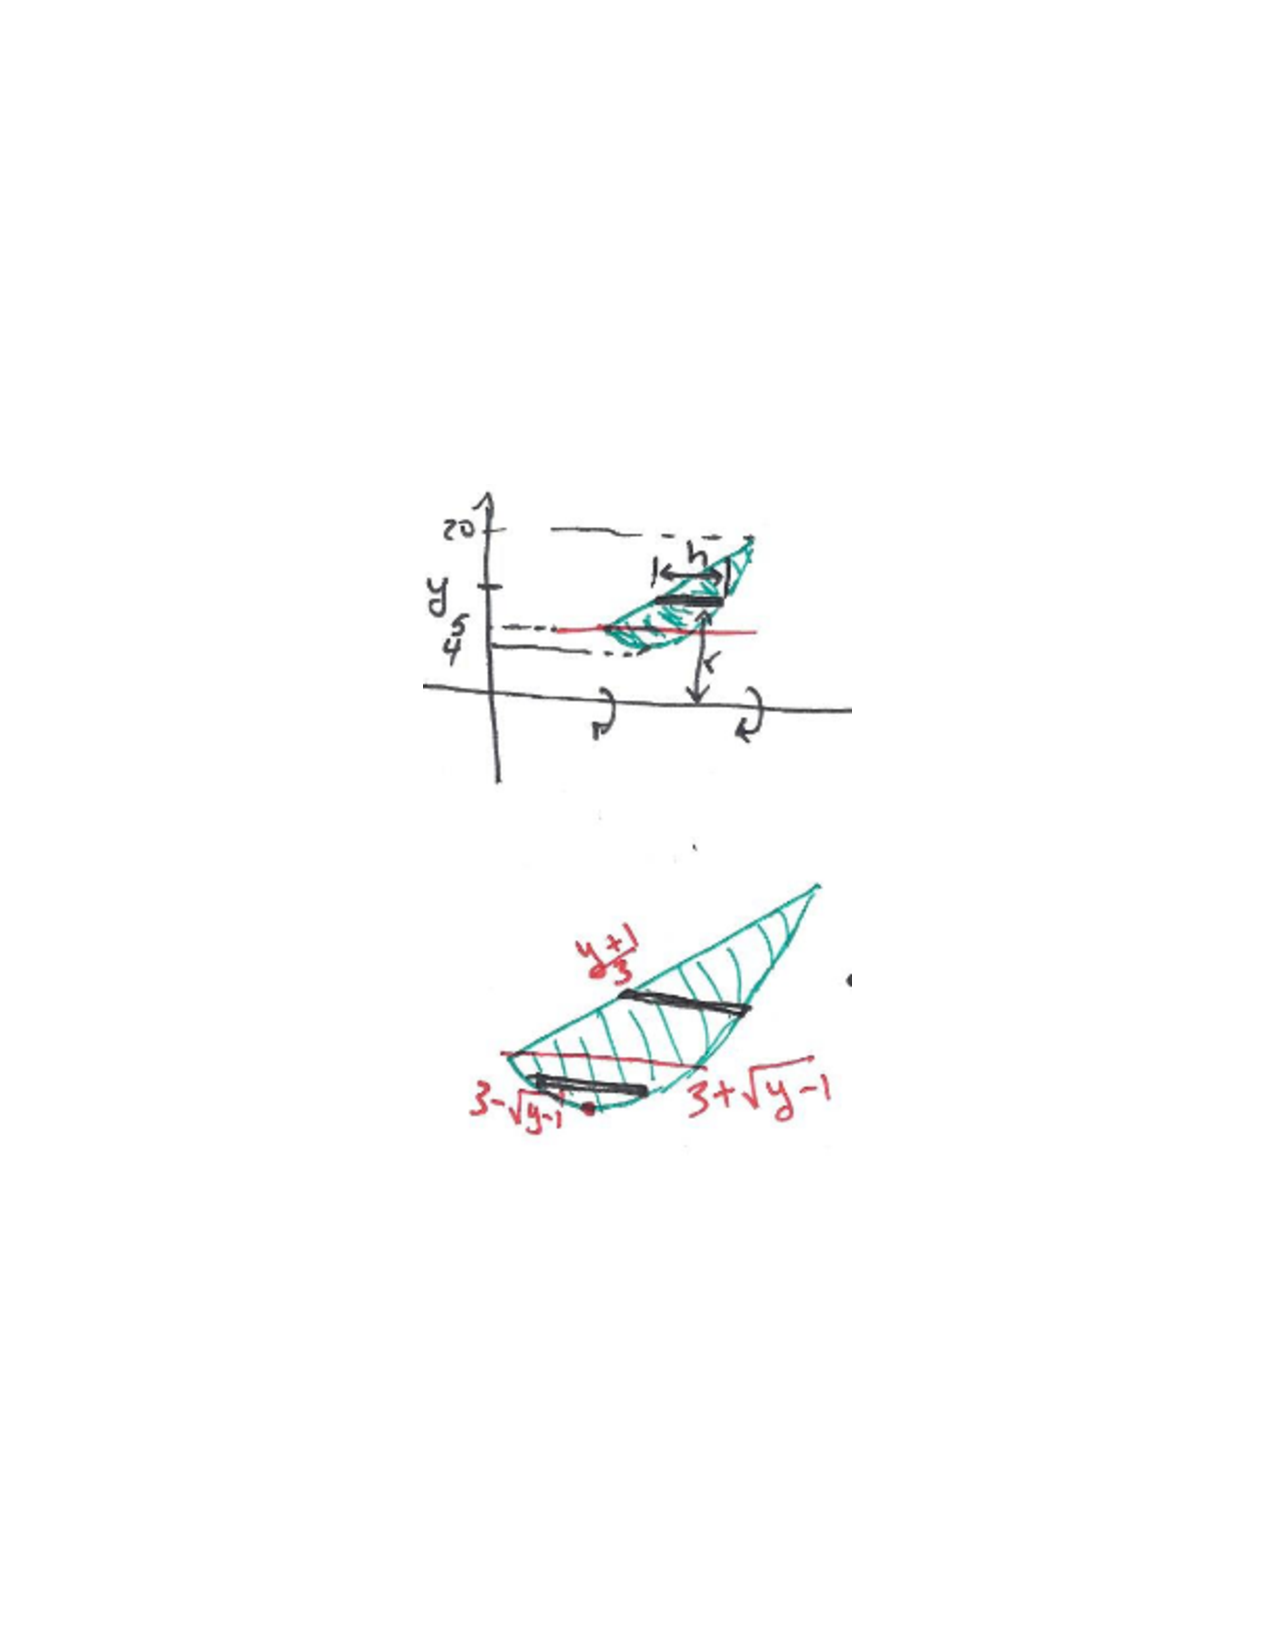
\includegraphics[trim= 200 240 150 240, scale=1]{Figure6-4-4.pdf}
		\end{image}
		
		It is pretty clear in this problem that the washer's method was easier than the shell's method.
		\end{freeResponse}
		
		
		
		\item  $y=-4$  
		\begin{freeResponse}
		{\bf Washers: }
		For washers, the cross-sections must be \dfn{perpendicular} to the axis of rotation.  
		So here we integrate along the $x$-axis.  
		We have that
			\begin{align*}
			r_{out} &= 4 + (3x-1) = 3x + 3 \\
			r_{in} &= 4 + (x^2 - 6x +13) = x^2 - 6x + 17
			\end{align*}
		and
			\[
			V = \pi \int_2^7 \left[ (3x+3)^2 - (x^2-6x+17)^2 \right] \d x.
			\]
		
		{\bf Shells: }
		For shells, the cross-sections must be \dfn{parallel} to the axis of rotation.  
		So here we integrate along the $y$-axis.
		Just as before though, the equation determining the bottom of the shell changes at $y=5$.  
		The height of the shell over the two regions is the same as part (a), but now the radius of the shell is $4+y$.
		So,
			\[
			V = 2\pi \left[ \int_4^5 (4+y) \cdot 2\sqrt{y-1} \d y + \int_5^{20} (4+y) \left( (3 + \sqrt{y+1}) - \frac{1}{3}(y+1) \right) \d y \right]
			\]
			
		\begin{image}
		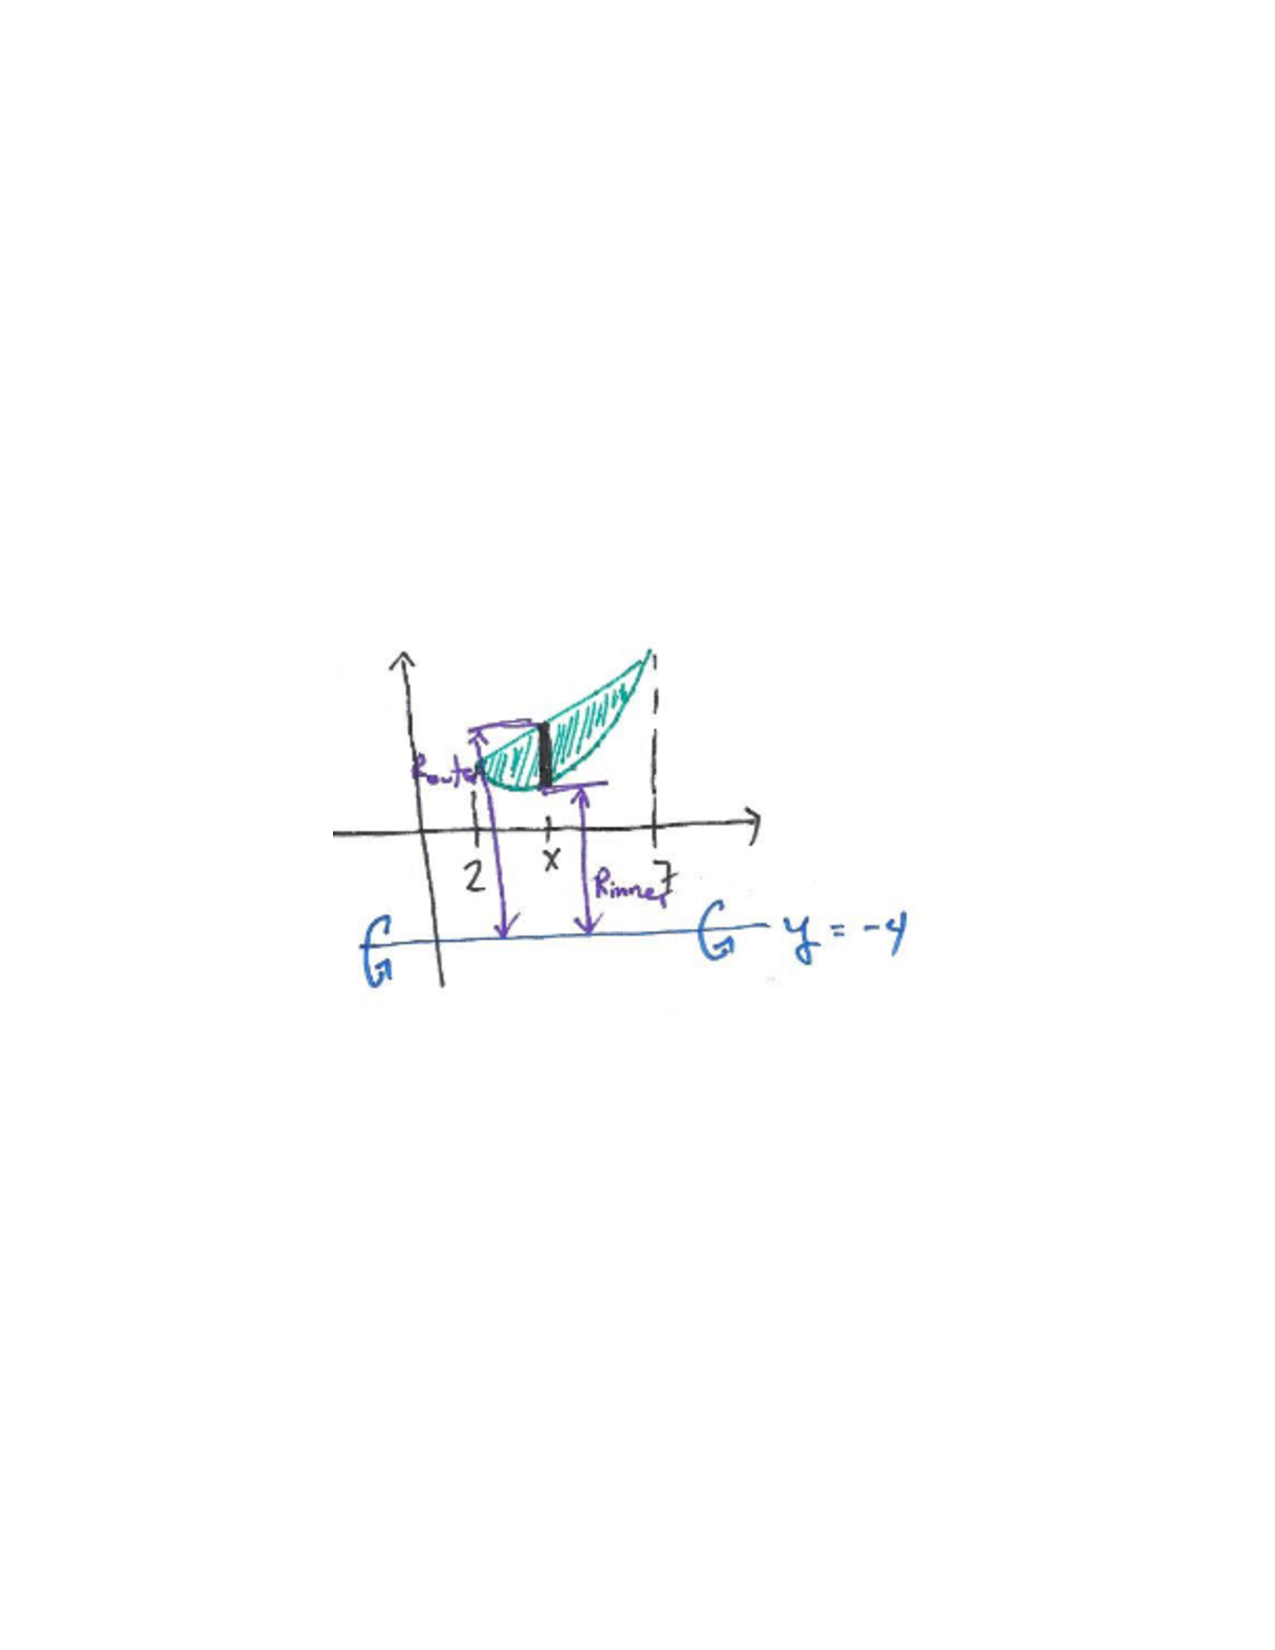
\includegraphics[trim= 150 320 150 310, scale=1]{Figure6-4-5.pdf}
		\end{image}
		
		Again, it is pretty clear that the washer's method was easier than the shell's method for this problem.
		\end{freeResponse}
		
		
		
		\item  $y=22$
		\begin{freeResponse}
		{\bf Washers: }
		For washers, the cross-sections must be perpendicular to the axis of rotation.  
		So here we integrate along the $x$-axis.  
		We have that
			\begin{align*}
			r_{out} &= 22 -  (x^2 - 6x +13) = -x^2 + 6x + 9 \\
			r_{in} &= 22 -  (3x-1) = -3x + 23
			\end{align*}
		and so
			\[
			V = \pi \int_2^7 \left[ (-x^2+6x+9)^2 - (-3x+23)^2 \right] \d x.
			\]

		{\bf Shells: }
		For shells, the cross-sections must be parallel to the axis of rotation.  
		So here we integrate along the $y$-axis.
		Just as before though, the equation determining the bottom of the shell changes at $y=5$.  
		The height of the shell over the two regions is the same as part (a), but now the radius of each shell is $22-y$.
		So,
			\[
			V = 2\pi \left[ \int_4^5 (22-y) \cdot 2\sqrt{y-1} \d y + \int_5^{20} (22-y) \left( (3 + \sqrt{y+1}) - \frac{1}{3}(y+1) \right) \d y \right]
			\]
			
		\begin{image}
		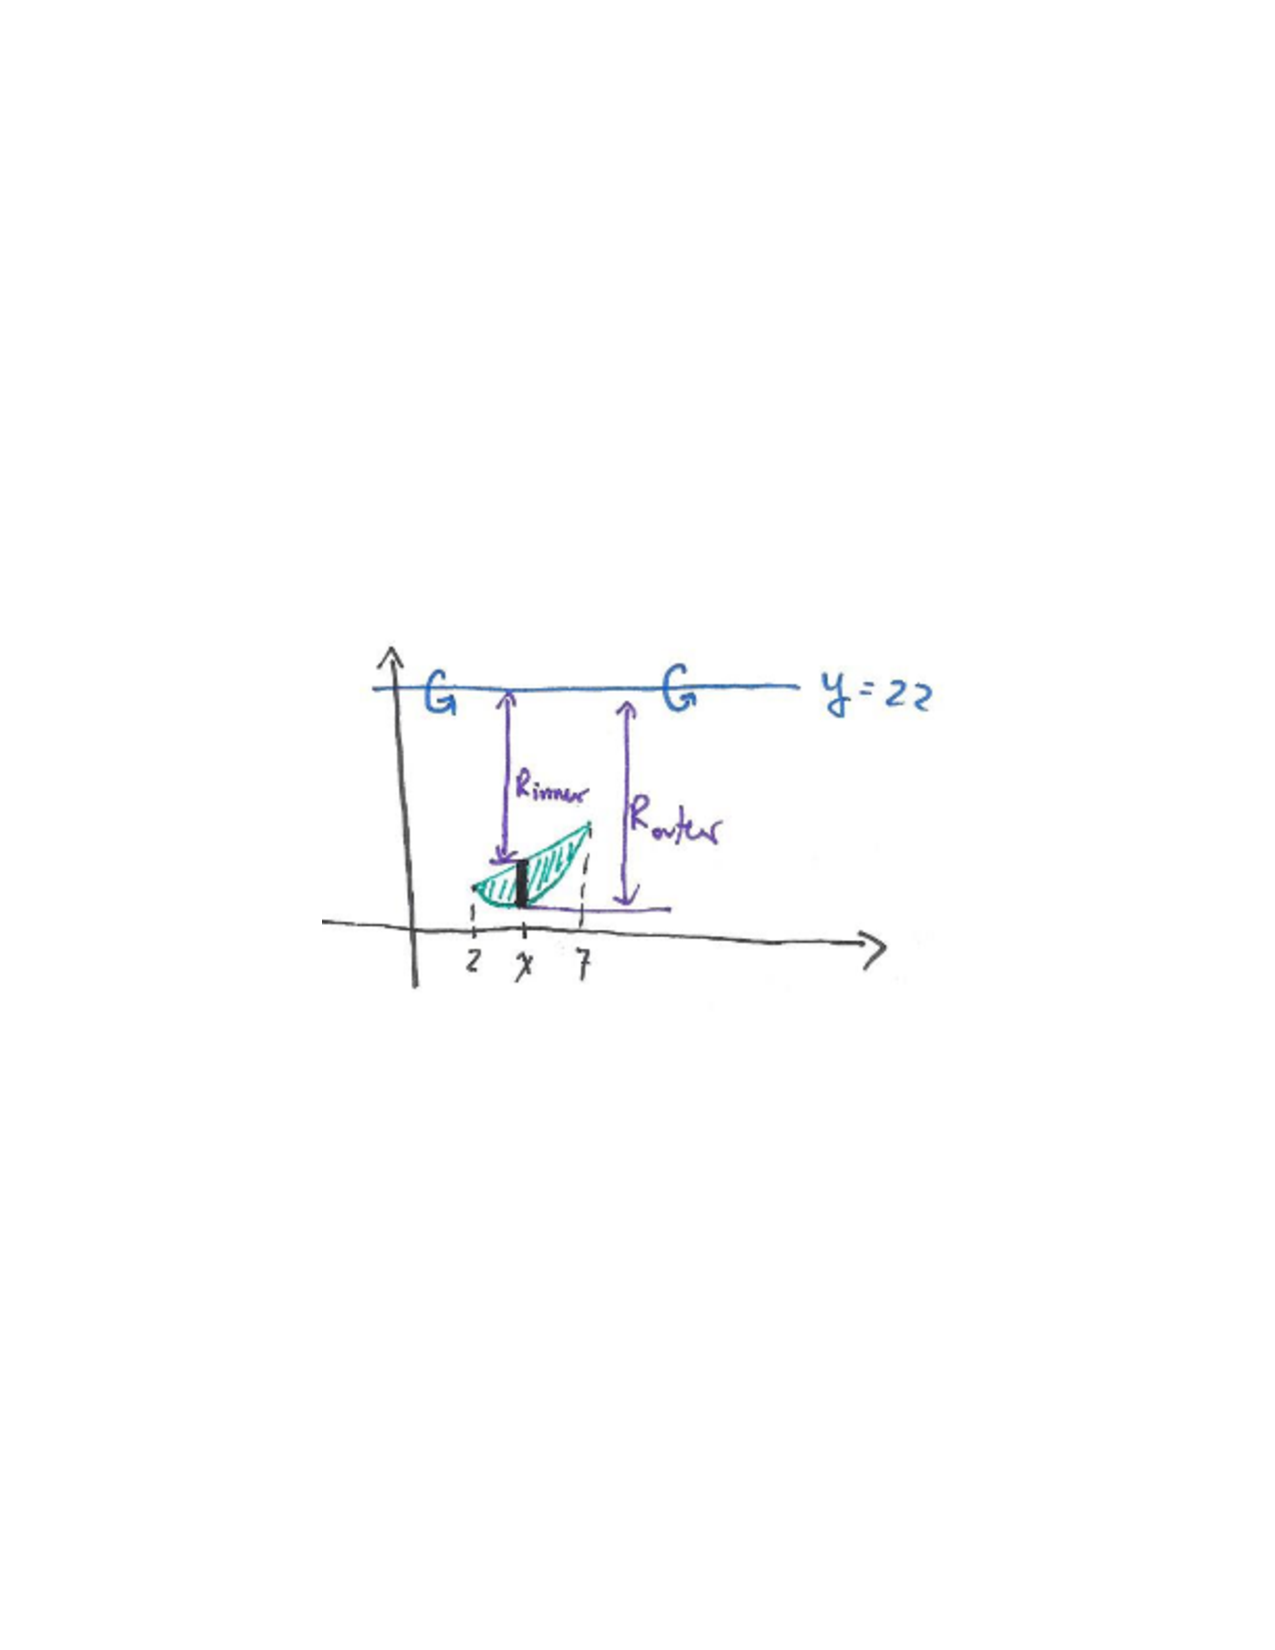
\includegraphics[trim= 150 320 150 310, scale=1]{Figure6-4-6.pdf}
		\end{image}
		
		Once again, the washer's method appears to be easier.
		\end{freeResponse}
		
		
		
		\item  the $y$-axis
		\begin{freeResponse}
		{\bf Washers: }
		For washers, the cross-sections must be perpendicular to the axis of rotation.  
		So here we integrate along the $y$-axis (notice the change from the three preceding problems).  
		Just as in the shells method for the previous three parts, we have to break up our region of integration at $y=5$.  
		We have the following two cases
			\begin{enumerate}
			\item[(1)]  for $4 \leq y \leq 5$
				\begin{align*}
				r_{out} &= 3+\sqrt{y-1} \\
				r_{in} &= 3-\sqrt{y-1}
				\end{align*}
			
			\item[(2)]  for $5 \leq y \leq 20$
				\begin{align*}
				r_{out} &= 3+\sqrt{y-1} \\
				r_{in} &= \frac{1}{3}(y+1)
				\end{align*}
			
			\end{enumerate}
		So,
			\[
			V = \pi \left[ \int_4^5 \left( \left(3+\sqrt{y-1} \right)^2 - \left(3-\sqrt{y-1}\right)^2 \right) \d y + \int_5^{20} \left( \left( 3+\sqrt{y-1} \right)^2 - \frac{1}{9}(y+1)^2 \right) \d y \right].
			\]
			
		\begin{image}
		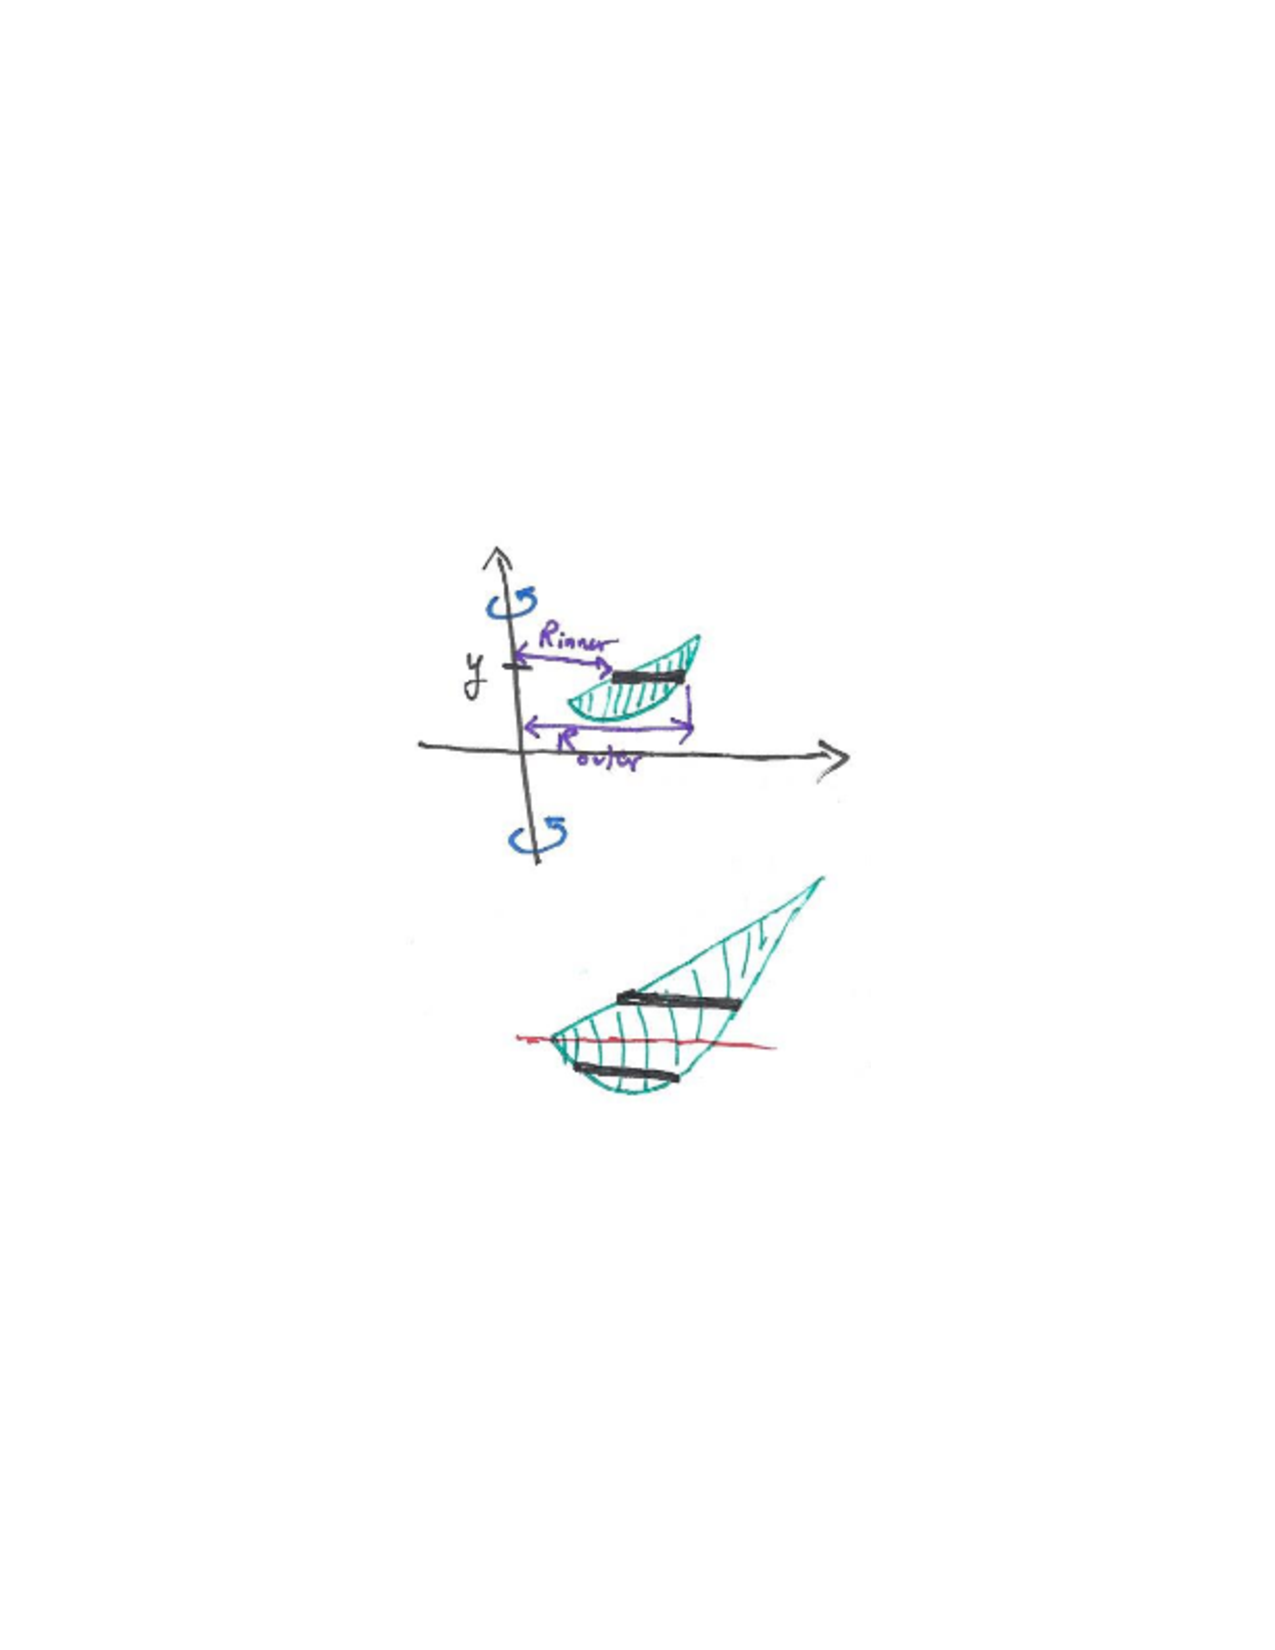
\includegraphics[trim= 150 270 150 270, scale=1]{Figure6-4-7.pdf}
		\end{image}

		{\bf Shells: }
		For shells, the cross-sections must be parallel to the axis of rotation.  
		So here we integrate along the $x$-axis (again, notice the change from the three preceding problems).
		This time, we do not need to break up the region!
		Our shells will always have the parameters
			\begin{align*}
			h &= (3x-1) - (x^2-6x+13) = -x^2+9x-14  \\
			r &= x
			\end{align*}
		So,
			\[
			V = 2 \pi \int_2^7 x (-x^2 + 9x - 14) \d x.
			\]
		\begin{image}
		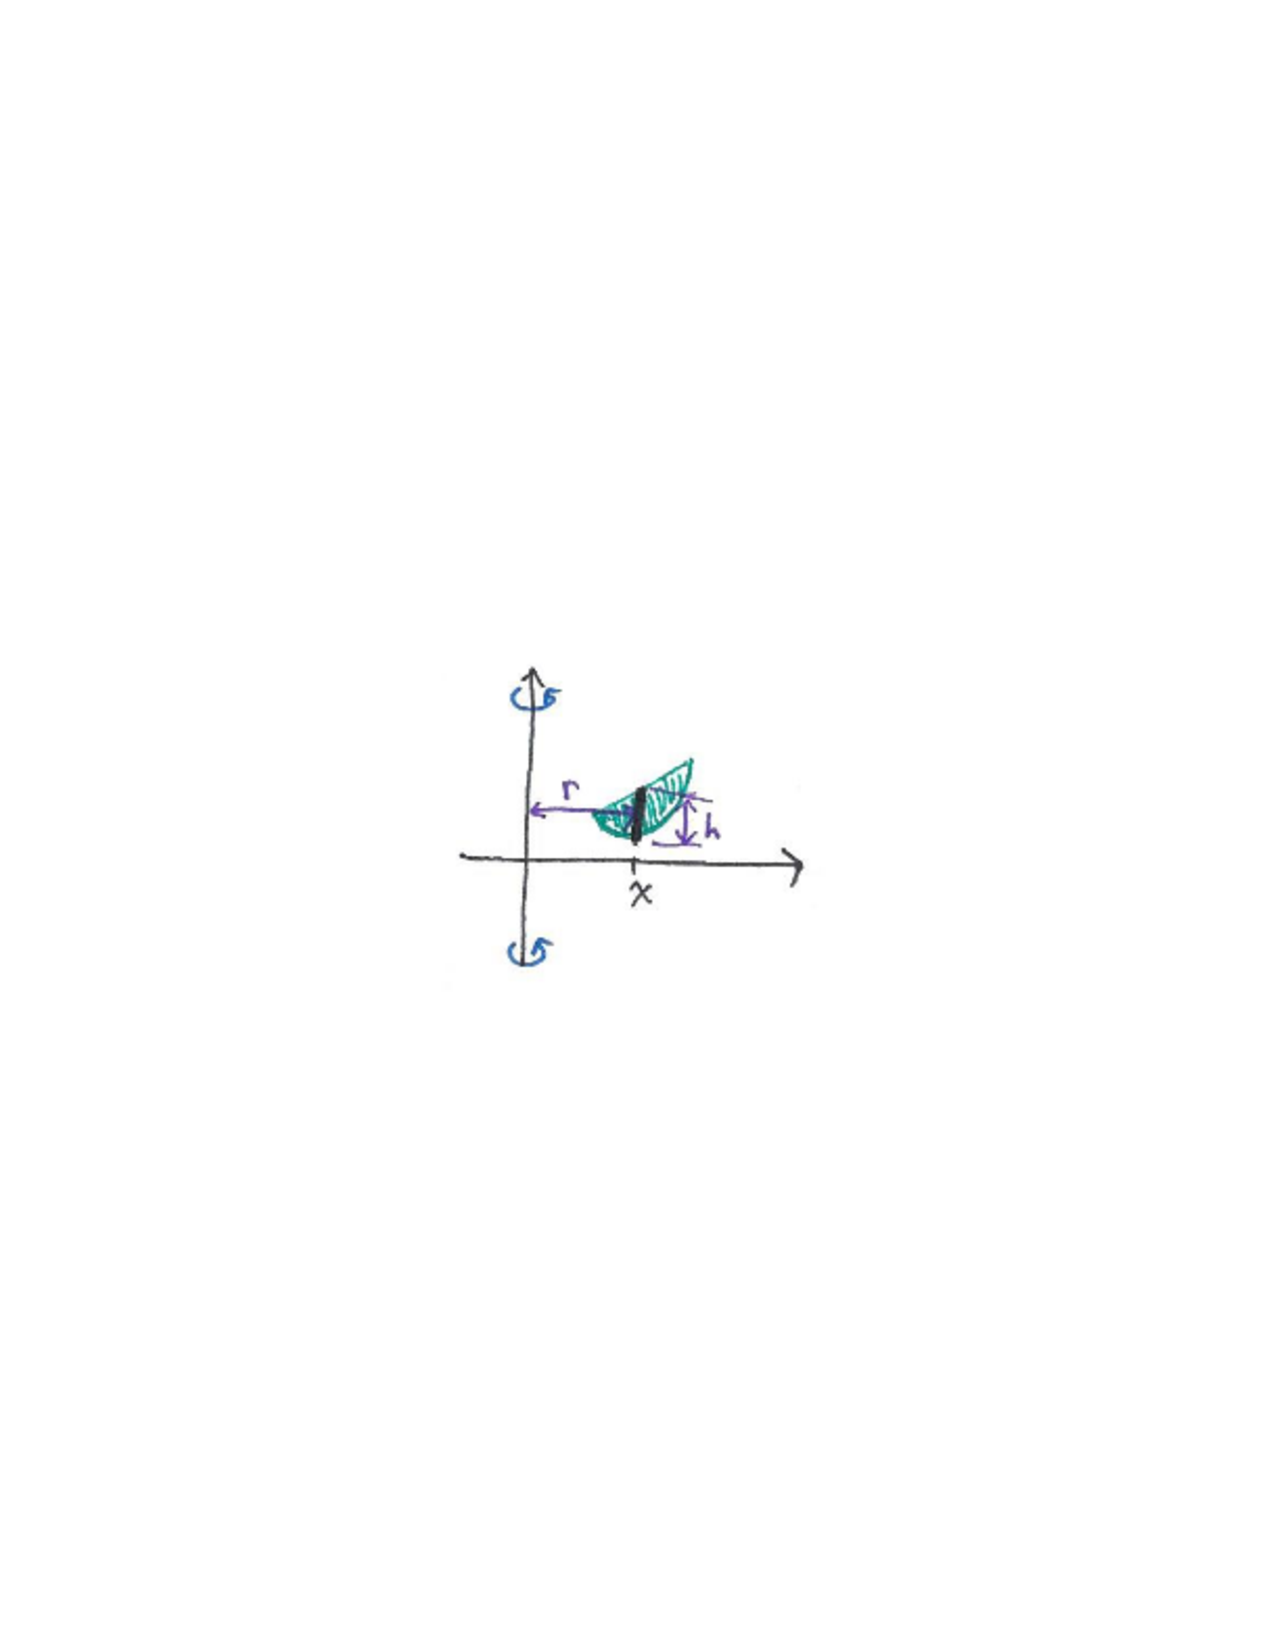
\includegraphics[trim= 150 320 150 310, scale=1]{Figure6-4-8.pdf}
		\end{image}
		
		Now, notice that the shells method was a lot easier.  
		The key for this region is that you want your cross sections to always be perpendicular to the $x$-axis.
		That way, the bounds for your parameters do not change over the entire region of integration.
		
		\end{freeResponse}
		
		
		
		\item  $x=-3$
		\begin{freeResponse}
		{\bf Washers: }
		For washers, the cross-sections must be perpendicular to the axis of rotation.  
		So here we integrate along the $y$-axis.
		Just as in part (d), we need to split the region up into two parts.  
		But shifting the axis of rotation to $x=-3$ just adds three to all radii.  
		So
			\[
			V = \pi \left[ \int_4^5 \left( \left(6+\sqrt{y-1} \right)^2 - \left(6-\sqrt{y-1}\right)^2 \right) \d y \right.
			\]
			\[
			+ \left. \int_5^{20} \left( \left( 6+\sqrt{y-1} \right)^2 - \left( 3 + \frac{1}{3}(y+1) \right)^2 \right) \d y \right].
			\]
			
		\begin{image}
		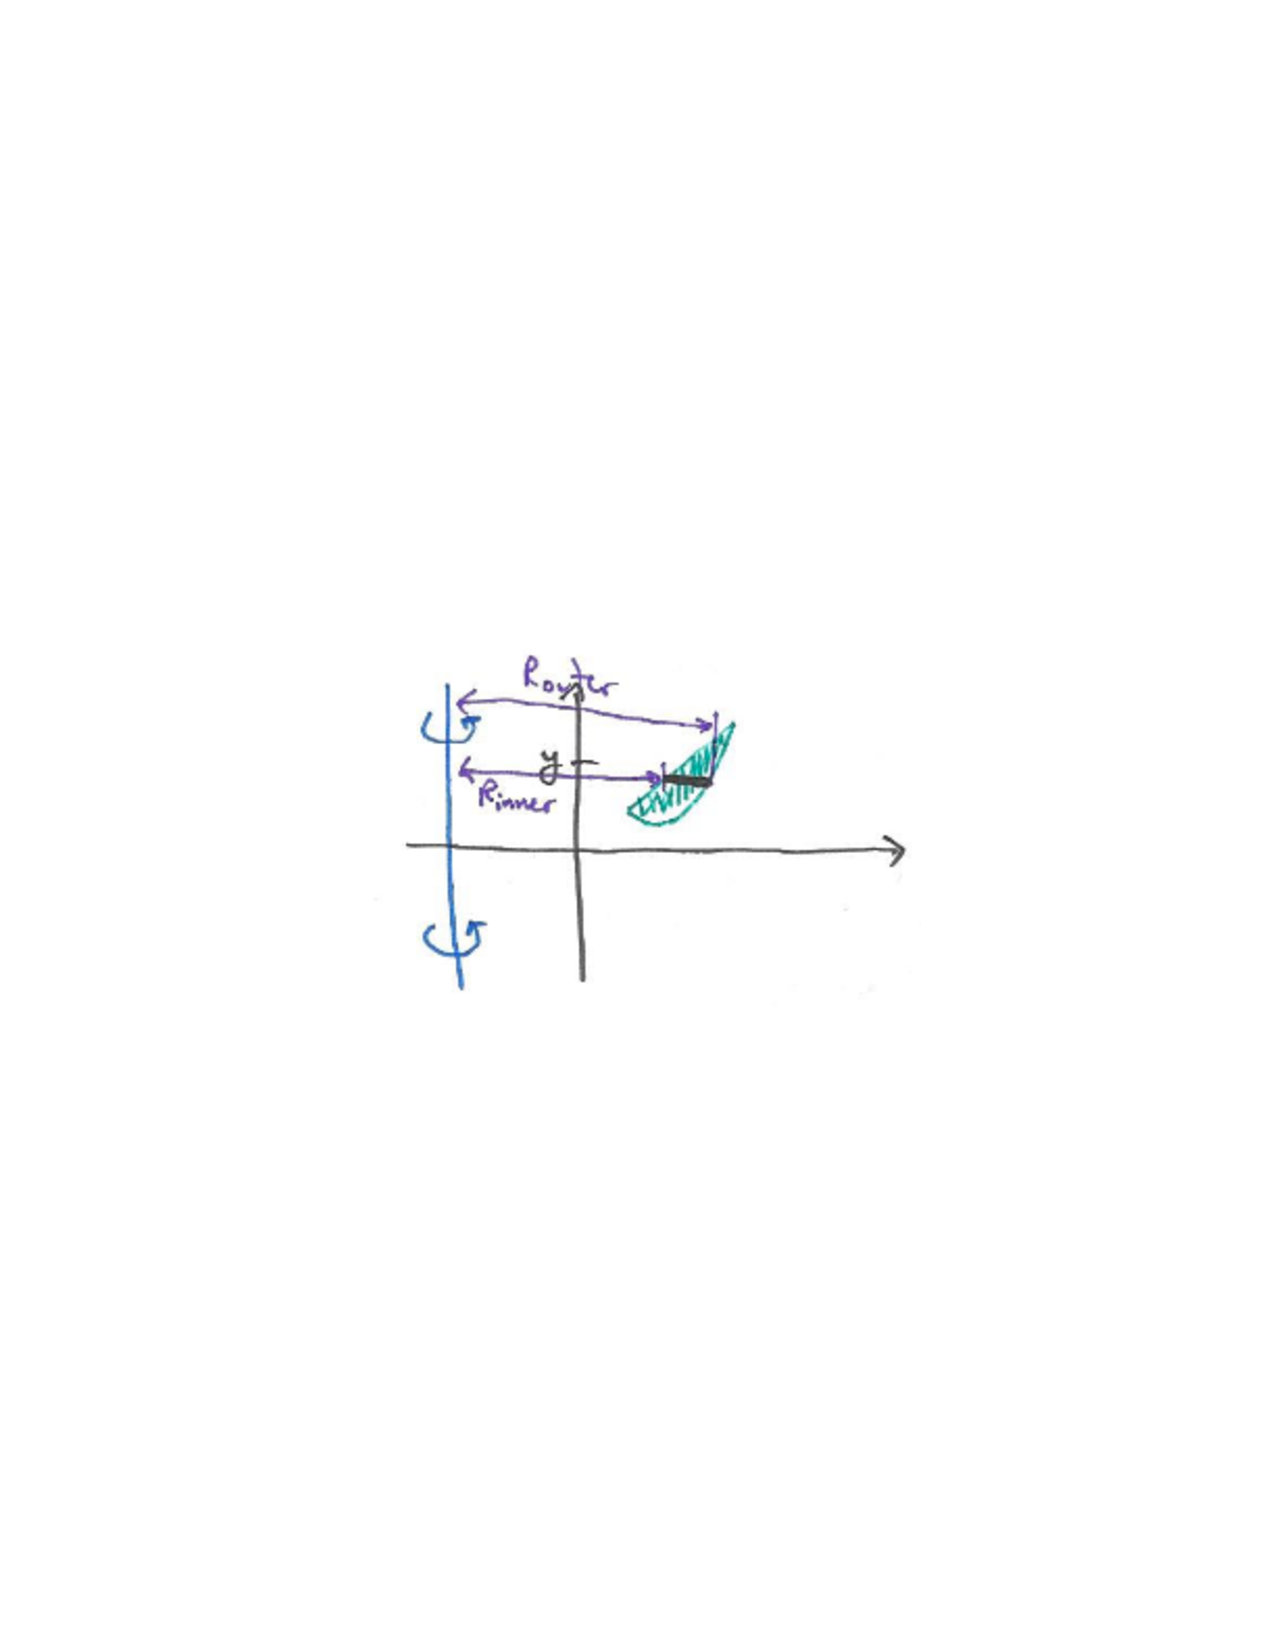
\includegraphics[trim= 150 320 150 310, scale=1]{Figure6-4-9.pdf}
		\end{image}
		
		{\bf Shells: }
		For shells, the cross-sections must be parallel to the axis of rotation.  
		So here we integrate along the $x$-axis.
		Shifting the axis of rotation to $x=-3$ simply adds three to the radius of the shell, so
			\[
			V = 2 \pi \int_2^7 (3+x) (-x^2 + 9x - 14) \d x.
			\]
			
		\begin{image}
		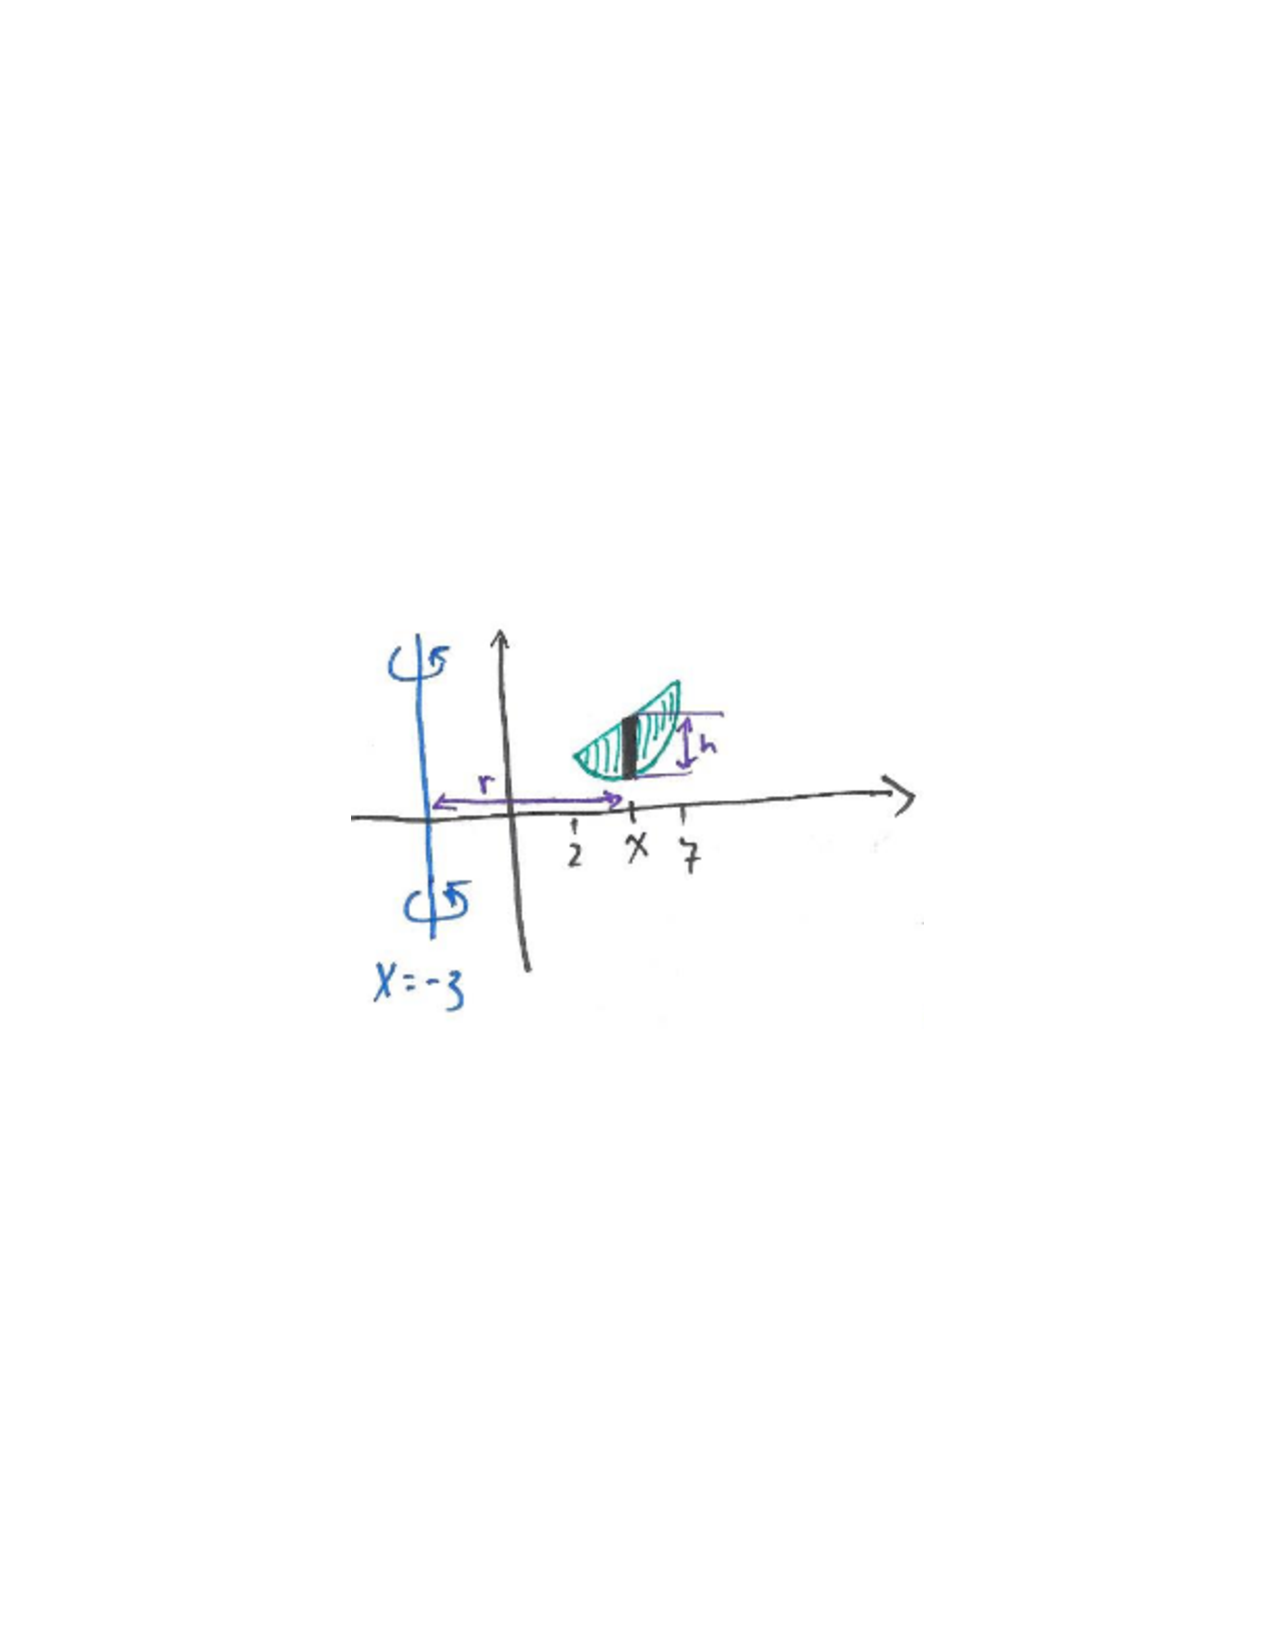
\includegraphics[trim= 150 320 150 310, scale=1]{Figure6-4-10.pdf}
		\end{image}
		
		The shells method was simpler.
		\end{freeResponse}
		
		
		
		\item$x=9$
		\begin{freeResponse}
		{\bf Washers: }
		For washers, the cross-sections must be perpendicular to the axis of rotation.  
		So here we integrate along the $y$-axis.
		Just as in parts (d) and (e), we need to split the region up into two parts.
		Via the figure below, we compute
			\begin{enumerate}
			\item[(1)]  for $4 \leq y \leq 5$
				\begin{align*}
				r_{out} &= 9-\left(3-\sqrt{y-1}\right) = 6+\sqrt{y-1} \\
				r_{in} &= 9-\left(3+\sqrt{y-1}\right) = 6-\sqrt{y-1}
				\end{align*}
			
			\item[(2)]  for $5 \leq y \leq 20$
				\begin{align*}
				r_{out} &= 9-\left( \frac{1}{3} (y+1) \right)  \\
				r_{in} &= 9-\left( 3+\sqrt{y-1} \right) = 6-\sqrt{y-1}
				\end{align*}
				
			\end{enumerate}
		So,
			\[
			V = \pi \left[ \int_4^5 \left( \left(6+\sqrt{y-1} \right)^2 - \left(6-\sqrt{y-1}\right)^2 \right) \d y \right.
			\]
			\[
			+ \left. \int_5^{20} \left( \left( 9 -  \frac{1}{3}(y+1) \right)^2 - \left( 6 - \sqrt{y-1} \right)^2 \right) \d y \right].
			\]
			
		\begin{image}
		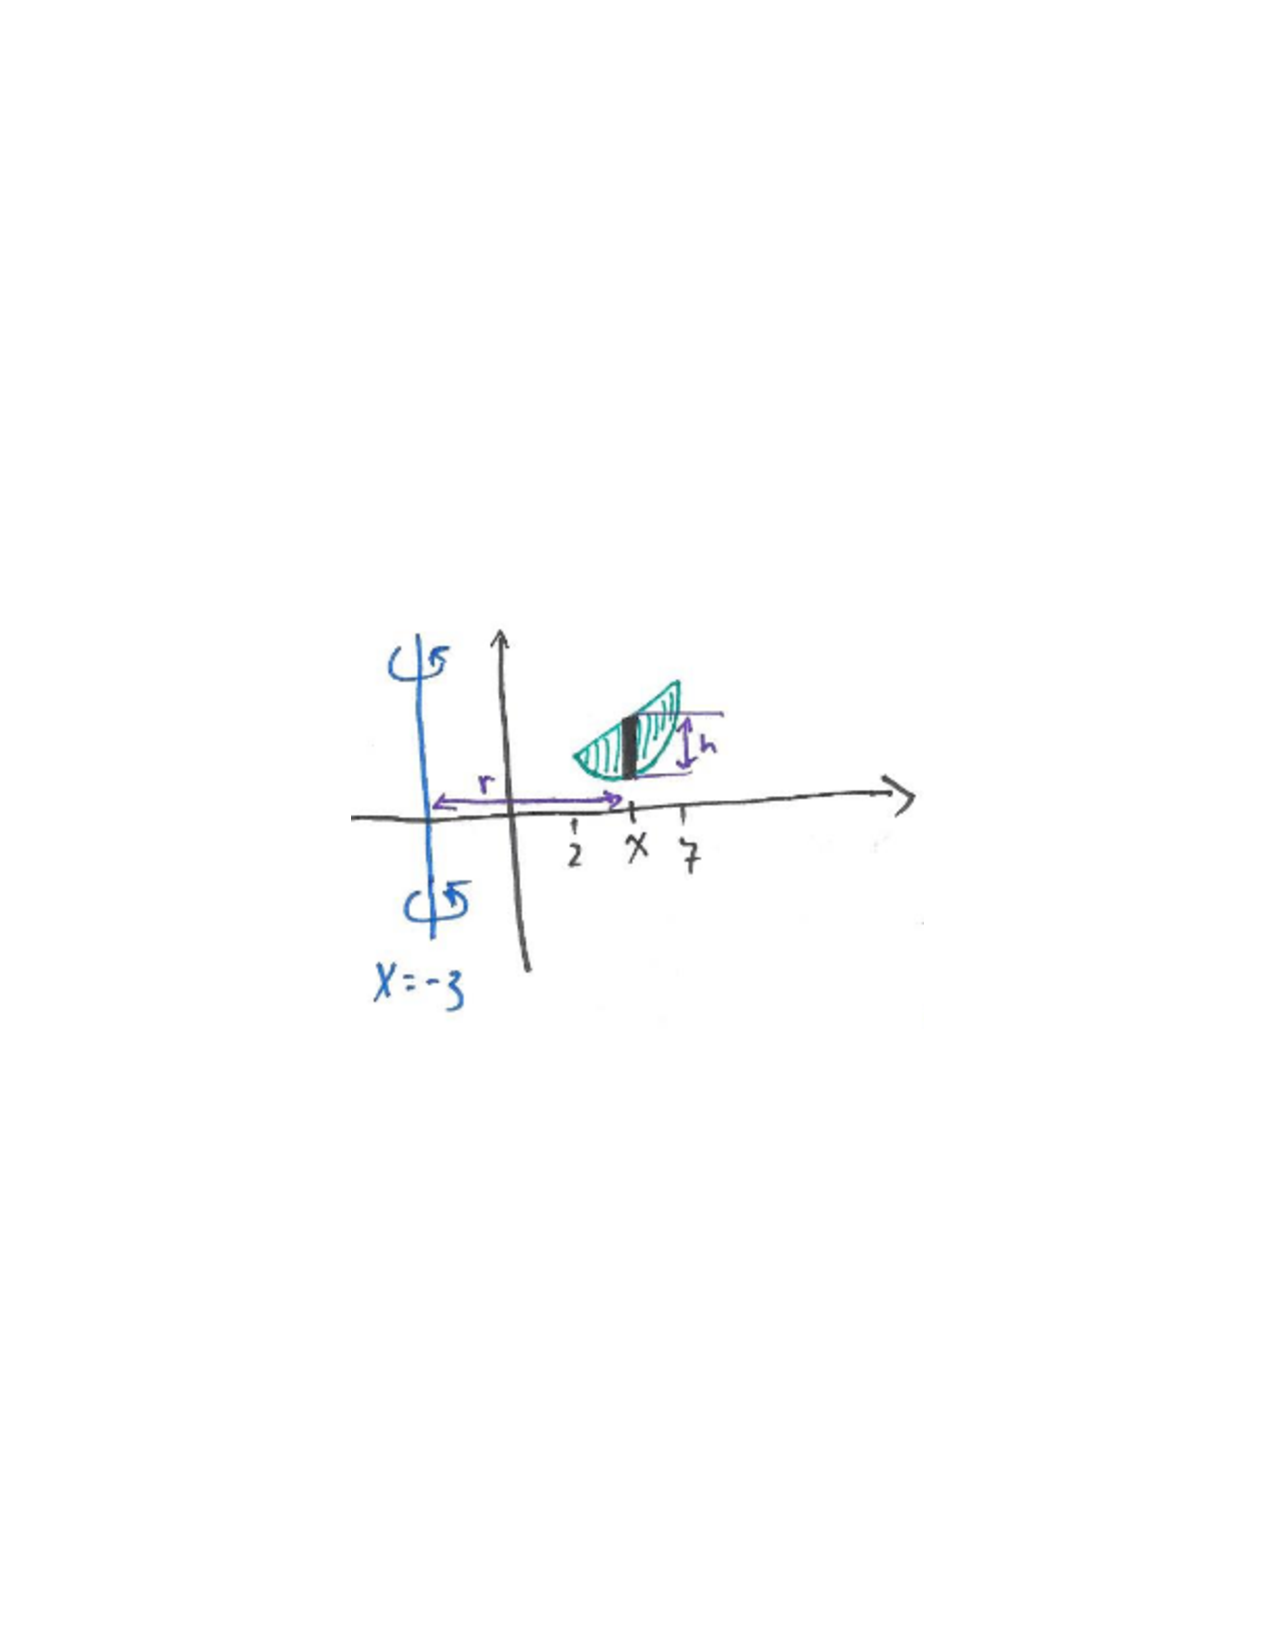
\includegraphics[trim= 150 310 150 300, scale=1]{Figure6-4-11.pdf}
		\end{image}
		
		{\bf Shells: }
		For shells, the cross-sections must be parallel to the axis of rotation.  
		So here we integrate along the $x$-axis.
		Shifting the axis of rotation to the right 9 units (from part (d)) does not change the height of the cylinder, and the radius changes to $9-x$.
		So
			\[
			V = 2 \pi \int_2^7 (9-x) (-x^2 + 9x - 14) \d x.
			\]
			
		\begin{image}
		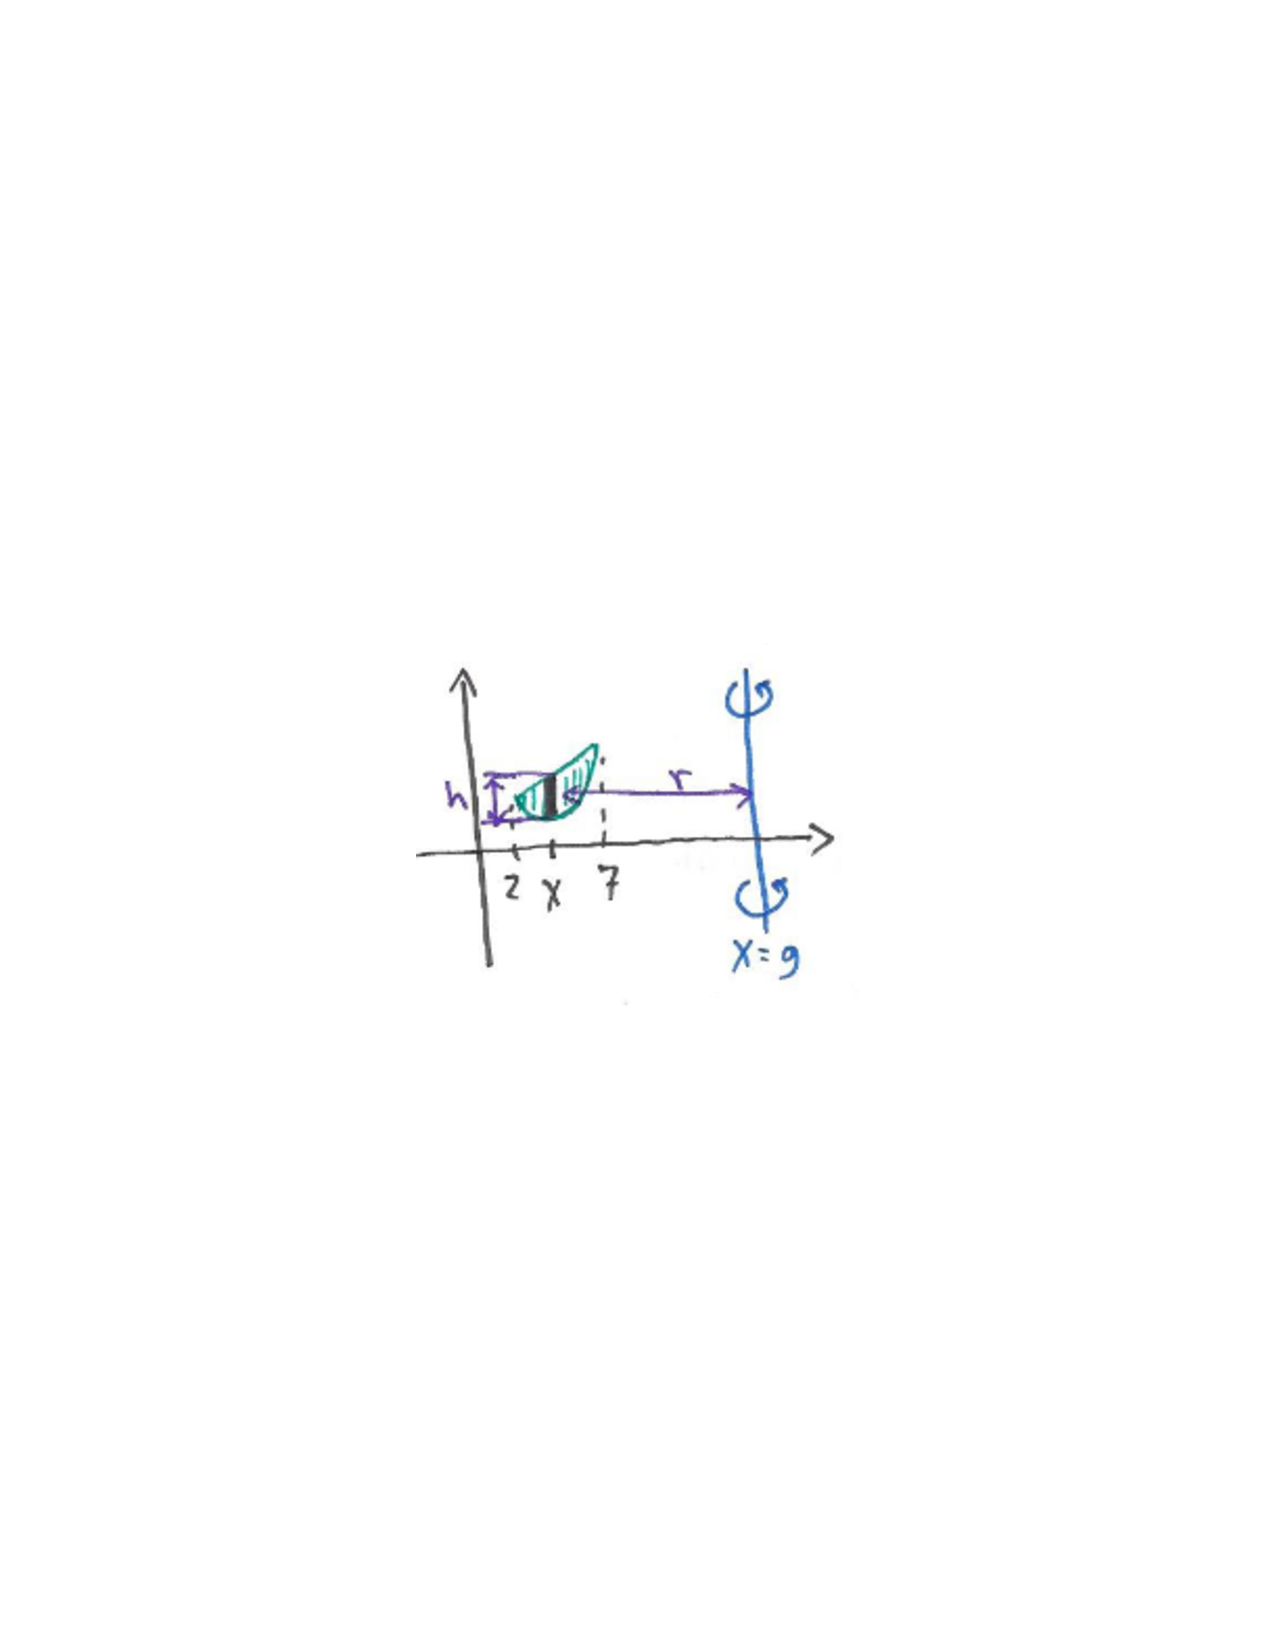
\includegraphics[trim= 150 310 150 300, scale=1]{Figure6-4-12.pdf}
		\end{image}
		
		Again, the shell method was much simpler.

		\end{freeResponse}
		
	\end{enumerate}
	
\end{problem}

\begin{instructorNotes}
Note that part (a) was on the Recitation \# 3 handout. Remind the students about the solution of part (a). 
For (b)-(e), split these between the groups. Allow time for group work and discussion.   
During the discussion, you might want to talk about all of the ``washer methods" before all of the ``shell methods".  
Be sure that they recognize (by the end) that we slice \dfn{perpendicular} to the axis of revolution in the washer method and \dfn{parallel} to the axis of revolution in the shell method.
\end{instructorNotes}



%problem 2
\begin{problem}
{\bf Set up} an integral (or a {\it sum of integrals}) to find the perimeter of the region bounded by the curves $y=2x^2-5x+13$ and $y=x^2+6x-11$.
	\begin{freeResponse}
	Let $f(x) = 2x^2-5x+13$ and $g(x) = x^2+6x-11$.
	We first need to find the points where these two curves intersect.  
	So we solve
		\begin{align*}
		f(x) &= g(x)  \\
		2x^2-5x+13 &= x^2+6x-11  \\
		x^2-11x+24 &= 0  \\
		(x-3)(x-8) &= 0  \\
		x &= 3,8.
		\end{align*}
	Then the perimeter is $L_1 + L_2$ where
		\begin{align*}
		L_1 &= \int_3^8 \sqrt{1+f'(x)^2} \d x = \int_3^8 \sqrt{1+(4x-5)^2} \d x  \\
		L_2 &= \int_3^8 \sqrt{1+g'(x)^2} \d x = \int_3^8 \sqrt{1+(2x+6)^2} \d x.
		\end{align*}	
	\end{freeResponse}
	
\end{problem}

\begin{instructorNotes}
It may be helpful to remind students that perimeter makes sense for more general two-dimensional shapes.
\end{instructorNotes}














%problem 3
\begin{problem}
A steady wind blows a kite due west.  
The kite's height above the ground from horizontal position $x=0$ ft. to $x=80$ ft. is given by
	\[
	y = 150 - \frac{1}{40}(x-50)^2.
	\]
Set up the integral to find the distance traveled by the kite.  
	\begin{freeResponse}
		\[
		\text{{\color{red} distance the kite traveled}} = \int_0^{80} \sqrt{1+y'(x)^2} \d x
		\]
	where $y(x) = 150 - \frac{1}{40}(x-50)^2$.  
	Then since $y' = - \frac{1}{20}(x-50)$, we have that
		\[
		\text{{\color{red} distance the kite traveled}} = \int_0^{80} \sqrt{1 + \frac{(x-50)^2}{400}} \d x.
		\]
	\end{freeResponse}
		
\end{problem}

\begin{instructorNotes}
After discussing the problem, you might ask what the difference is between the given problem and if, say we are given the height of a ball at any time $t$ and asked to find the distance that the ball traveled.  
In this set-up, the height is not the \dfn{path} of the ball and thus the length of the curve does not represent the distance that the ball traveled.  
\end{instructorNotes}


















	
	
	
	
	
	
	
	
	

	










								
				
				
	














\end{document} 


















